% Praktická část: porovnání rozhraní aplikace s doporučeními z kapitoly
% kap:uzivatelske-rozhrani. Vkládá se do kapitoly 07-navrh.tex.
% Stav odpovídá aplikaci k 23. 11. 2026 (po PR #69).
\section{Návrh uživatelského rozhraní a~jeho soulad se zásadami}\label{sec:ui-soulad}

Tento oddíl porovnává rozhraní aplikace se zásadami z~kapitoly~\ref{kap:uzivatelske-rozhrani}. U~každého návrhového rozhodnutí uvádí, o~které doporučení se opírá a~zda ho aplikace splňuje. Úpravy, které porovnání vyvolalo, popisuje konec oddílu.

\subsection{Rozvržení obrazovky}

Obrazovka aplikace má tři pevné části. Nahoře je lišta s~logem a~názvem aplikace, přepínačem světlého a~tmavého režimu, jménem přihlášeného uživatele a~tlačítkem pro odhlášení. Vlevo je svislá navigace s~hlavními částmi aplikace: Pracovní plocha, Zakázky, Zákazníci, Zařízení, Dokumenty, Kalendář a~(jen pro uživatele s~oprávněním Nastavení) Nastavení. Zbytek obrazovky zabírá obsah zvolené části. Nad obsahem je drobečková navigace, která ukazuje, kde se uživatel nachází.

Svislá navigace vlevo odpovídá doporučení Laubheimera: svislý seznam se rychle prohlíží a~lze do něj přidávat další položky \cite{Laubheimer2021}. To je pro aplikaci důležité, protože každý nový modul přidá do navigace novou položku. Navigaci lze sbalit jen na ikony, což Laubheimer připouští u~aplikací používaných denně. Ve výchozím stavu jsou proto vidět ikony i~textové popisky.

\subsection{Přehled rozhodnutí}

Tabulka~\ref{tab:ui-soulad} shrnuje hlavní rozhodnutí o~rozhraní a~jejich oporu v~literatuře.

\begin{longtable}{p{0.34\textwidth}p{0.40\textwidth}p{0.16\textwidth}}
\caption{Rozhodnutí o~uživatelském rozhraní a~jejich opora}\label{tab:ui-soulad}\\
\hline \textbf{Rozhodnutí} & \textbf{Opora} & \textbf{Stav} \\ \hline\endfirsthead
\hline \textbf{Rozhodnutí} & \textbf{Opora} & \textbf{Stav} \\ \hline\endhead
Hlavní menu je svislá lišta vlevo s~ikonou a~textem & svislá navigace vlevo se snadno prohlíží a~rozšiřuje \cite{Laubheimer2021} & splňuje \\
Lištu lze sbalit jen na ikony & přijatelné u~aplikací používaných denně \cite{Laubheimer2021} & splňuje \\
Tlačítko \enquote{+ Nový} je u~všech seznamů na stejném místě vpravo nahoře & hlavní akce na stejném místě v~pravém horním rohu \cite{Kaplan2021}; konzistence \cite[s.~2328]{Sajedi2011}; Fittsův zákon \cite[s.~2330]{Sajedi2011} & splňuje \\
Všechny seznamy mají stejnou tabulku, hledání a~řazení & konzistence \cite{Nielsen-heuristiky}, \cite{Shneiderman-pravidla}, \cite[s.~2328]{Sajedi2011} & splňuje \\
Postup v~aplikaci kopíruje postup ve firmě & shoda s~reálným světem \cite{Nielsen-heuristiky}; cyklus událostí \cite[s.~56]{MonkWagner2013} & splňuje \\
Nabídka a~faktura se skládají z~uložených dat zakázky & faktura vzniká kopírováním dat objednávky \cite[s.~57]{MonkWagner2013}; systém doplňuje známé údaje \cite[s.~2331--2332]{Sajedi2011} & splňuje \\
Vše o~zakázce na jedné obrazovce se záložkami & snížit zátěž krátkodobé paměti \cite{Shneiderman-pravidla}; jednoduché propojené formuláře \cite[s.~2330]{Sajedi2011} & splňuje \\
Výběr zákazníka, zařízení a~materiálu našeptávačem s~možností založit nový záznam & prevence chyb, rozpoznání místo vybavování \cite{Nielsen-heuristiky} & splňuje \\
Pracovní plocha s~naposledy otevřenými a~otevřenými zakázkami & rozpoznání místo vybavování \cite{Nielsen-heuristiky}; systém si pamatuje volby \cite[s.~2331--2332]{Sajedi2011} & splňuje \\
Drobečková navigace a~zvýrazněná položka menu & viditelnost stavu systému \cite{Nielsen-heuristiky}; navigace \cite[s.~2332--2333]{Sajedi2011} & splňuje \\
Hlášení po uložení nebo smazání & informativní zpětná vazba \cite{Shneiderman-pravidla} & splňuje \\
Záznamy s~historií se jen deaktivují, změny se zapisují do historie & snadné vrácení akcí \cite{Shneiderman-pravidla}; nouzový východ \cite[s.~2331]{Sajedi2011} & splňuje \\
Nastavení a~šablony vidí jen uživatel s~oprávněním Nastavení, ostatní tlačítka se skrývají podle role & postupné odhalování \cite{Nielsen-progressive}; skrýt funkce podle oprávnění \cite[s.~2331]{Sajedi2011} & splňuje \\
Stav zakázky má barvu (volitelnou v~nastavení) i~text & barva jen jako doplněk \cite[s.~2329]{Sajedi2011}; WCAG 1.4.1 \cite{WCAG22} & splňuje \\
Aplikace obsahuje jen funkce, které firma potřebuje & minimalistický design \cite{Nielsen-heuristiky}; skrýt informace navíc \cite[s.~2332]{Sajedi2011} & splňuje \\
Na stránce zakázky je zvýrazněn jeden doporučený další krok, ostatní tlačítka jsou ve skupinách & minimalismus a~hierarchie \cite{Nielsen-heuristiky}, \cite{Kaplan2021}; dialogy s~jasným zakončením \cite{Shneiderman-pravidla} & splňuje \\
Nápověda u~složitějších formulářů & nápověda \cite[s.~2330]{Sajedi2011}, \cite{Nielsen-heuristiky} & splňuje \\
Kontrast textu a~velikost klikacích prvků & WCAG 1.4.3 a~2.5.8 \cite{WCAG22} & splňuje \\
Nevratné akce se potvrzují v~okně aplikace s~jasnou otázkou a~pojmenovaným tlačítkem & předcházet chybám \cite{Shneiderman-pravidla}; potvrzení nevratné akce \cite[s.~2331--2332]{Sajedi2011} & splňuje \\
Chybný údaj ve formuláři se hlásí česky u~políčka s~příkladem správného zápisu & pomoc s~rozpoznáním a~opravou chyb \cite{Nielsen-heuristiky} & splňuje \\
\hline
\end{longtable}

\subsection{Inspirace z~rešerše}\label{sec:ui-inspirace}

Při návrhu seznamů aplikace byly využity podněty z~rešerše (oddíl~\ref{sec:reserse-inspirace}). Všechny vycházejí z~požadavku na konzistenci rozhraní \cite{Nielsen-heuristiky}, \cite[s.~2328]{Sajedi2011}, který rešerše potvrdila: jednotné rozložení obrazovky bylo pozitivně hodnoceno u~Odoo i~ABRA Flexi.

\paragraph{Jednotné rozložení seznamů.} Všechny sekce mají stejnou hlavičku: vlevo název a~počet záznamů, vpravo hlavní akce. Pod ní je lišta, ve které je vyhledávací pole vždy na prvním místě a~ve stejné šířce, za ním filtry a~vpravo přepínač zobrazení. Sloupce tabulky mají pevnou šířku, takže se po filtrování ani hledání nepřeskupí a~uživatel nemusí znovu hledat, kde je který údaj.

\paragraph{Okno Filtrovat a~souhrn dokladů.} Seznam zakázek, seznam zařízení a~kalendář mají vedle vyhledávacího pole tlačítko \enquote{Filtrovat} (obrázek~\ref{obr:bm-filtr-stavu}). Otevře okno, ve kterém uživatel zaškrtne, co chce vidět: stavy s~počtem záznamů v~každém z~nich (u~zařízení stav jejich poslední zakázky), v~kalendáři typy událostí a~zaměstnance. U~zakázek v~něm zvolí i~řazení podle data přijetí nebo vydání. Tlačítko ukazuje počet zvolených filtrů a~vedle něj jsou štítky aktivních filtrů, které lze jedním kliknutím odebrat, takže je stále vidět, co je vyfiltrováno \cite{Nielsen-heuristiky}. Sekce Dokumenty má nad tabulkou řádek typů dokumentů s~počty, mezi kterými se přepíná jako mezi záložkami. Pod tabulkou dokumentů je navíc souhrn počtu a~celkové částky dokladů, inspirovaný ABRA Flexi.

\paragraph{Kanbanové zobrazení (Odoo).} Seznam zákazníků, zařízení a~zakázek lze přepnout z~tabulky na karty (obrázky~\ref{obr:odoo-prepinac} a~\ref{obr:bm-kanban}). Karta obsahuje jen základní údaje, podobně jako kanban kontaktů v~Odoo. Zakázky jsou v~kanbanu rozdělené do sloupců podle stavu, takže je na první pohled vidět, kolik práce čeká v~jaké fázi. Aplikace si zvolené zobrazení pamatuje zvlášť pro každý seznam.

\begin{figure}[h]
\centering
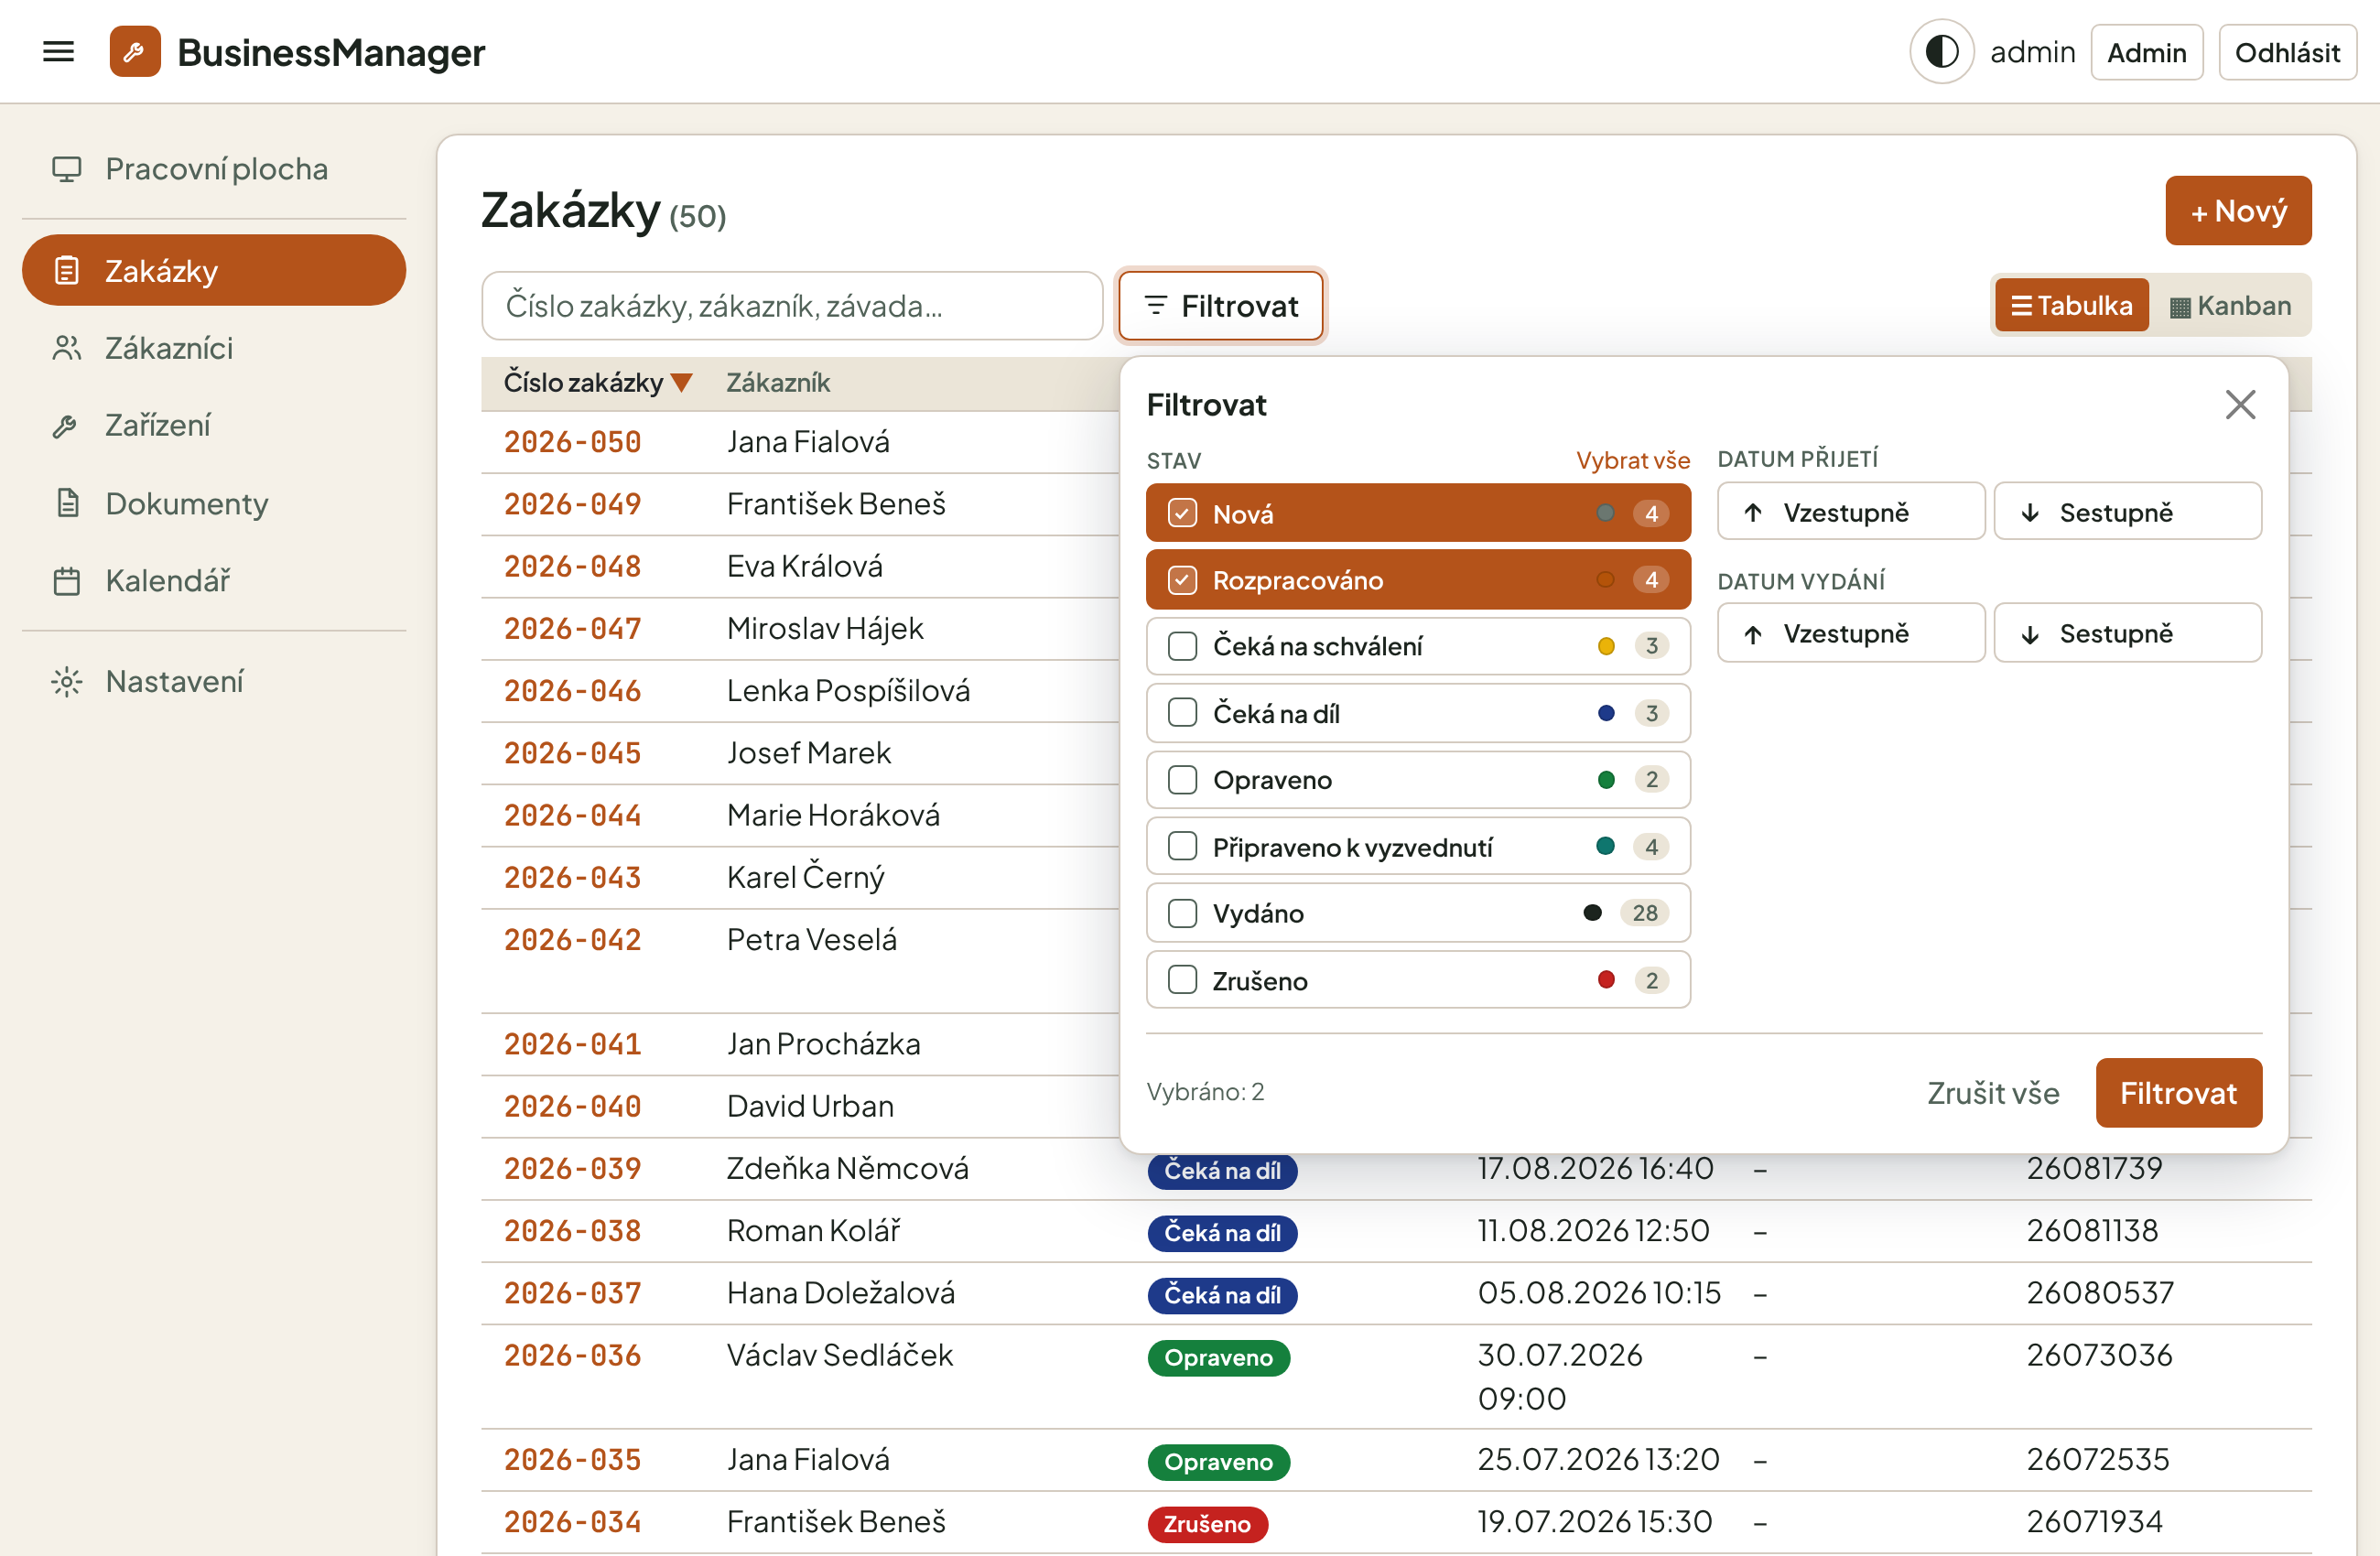
\includegraphics[width=\linewidth]{obrazky/navrh/bm-zakazky-filtr.png}
\caption{Seznam zakázek v~aplikaci s~otevřeným oknem Filtrovat, stavy s~počty záznamů a~řazením podle data (zdroj: vlastní)}\label{obr:bm-filtr-stavu}
\end{figure}

\begin{figure}[h]
\centering
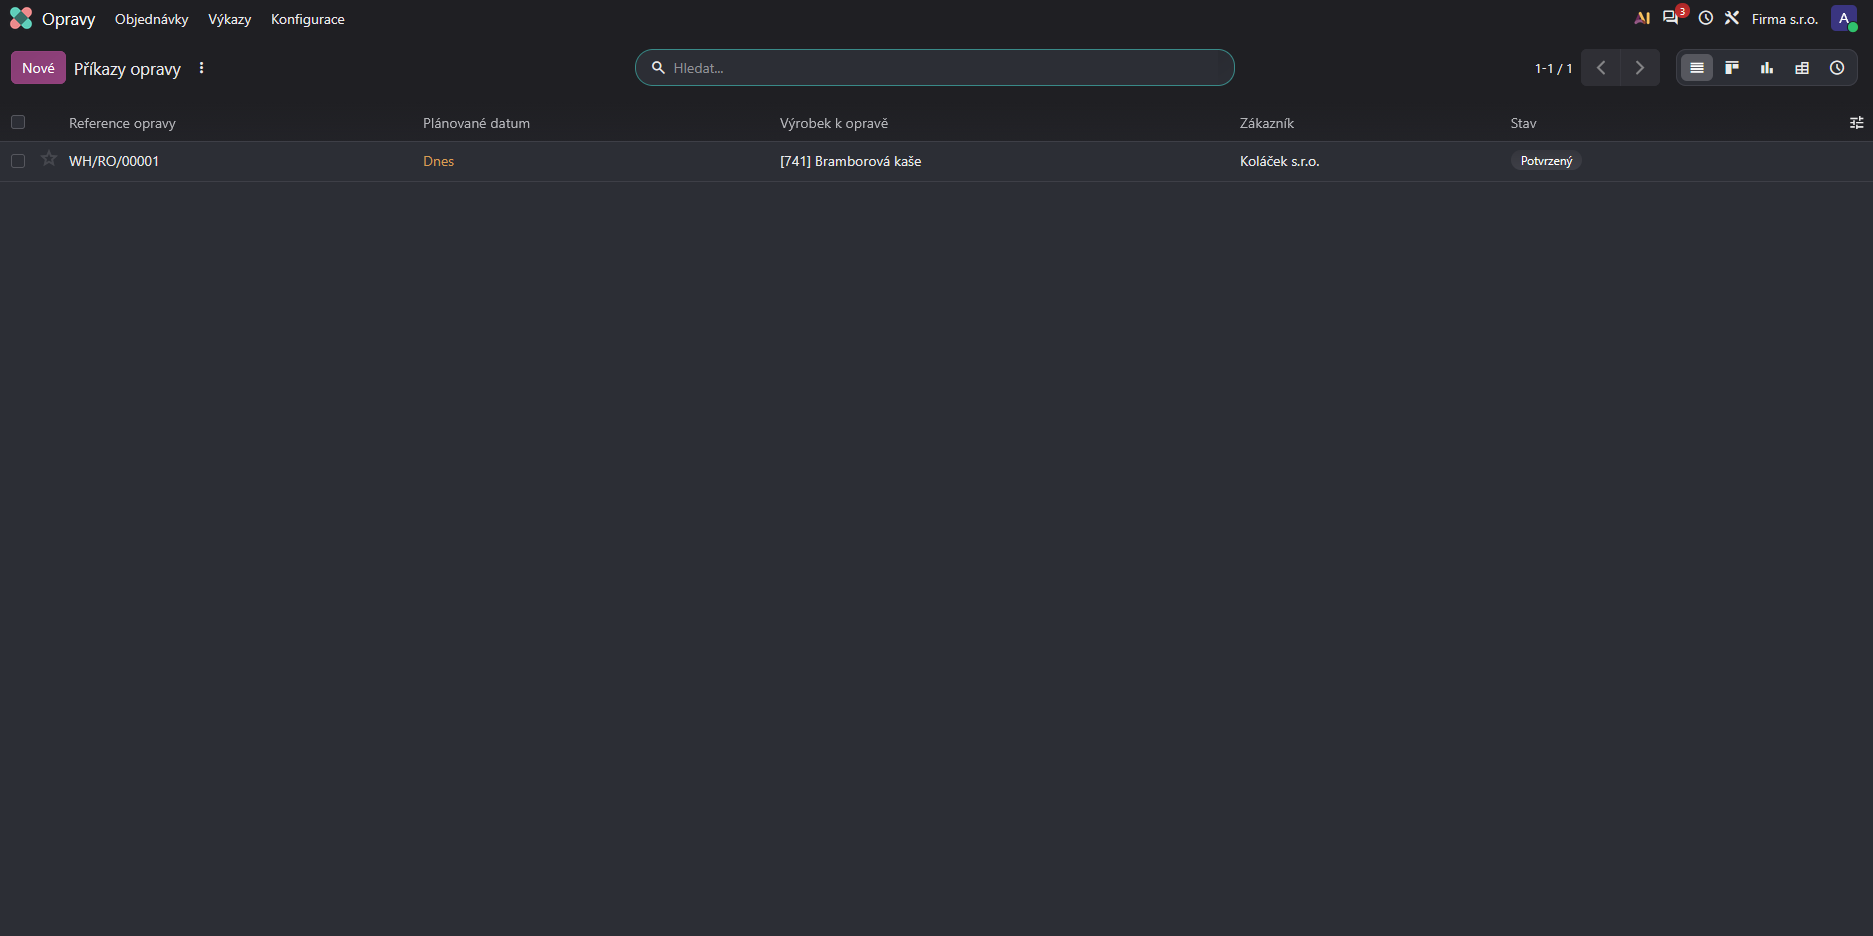
\includegraphics[width=\linewidth]{obrazky/reserse/odoo_strana_opravy.png}
\caption{Seznam oprav v~Odoo s~přepínačem zobrazení vpravo nahoře (seznam, kanban, graf, pivot, aktivity) (zdroj: vlastní snímek obrazovky ze zkušební verze, pořízeno 3.~11.~2026)}\label{obr:odoo-prepinac}
\end{figure}

\begin{figure}[h]
\centering
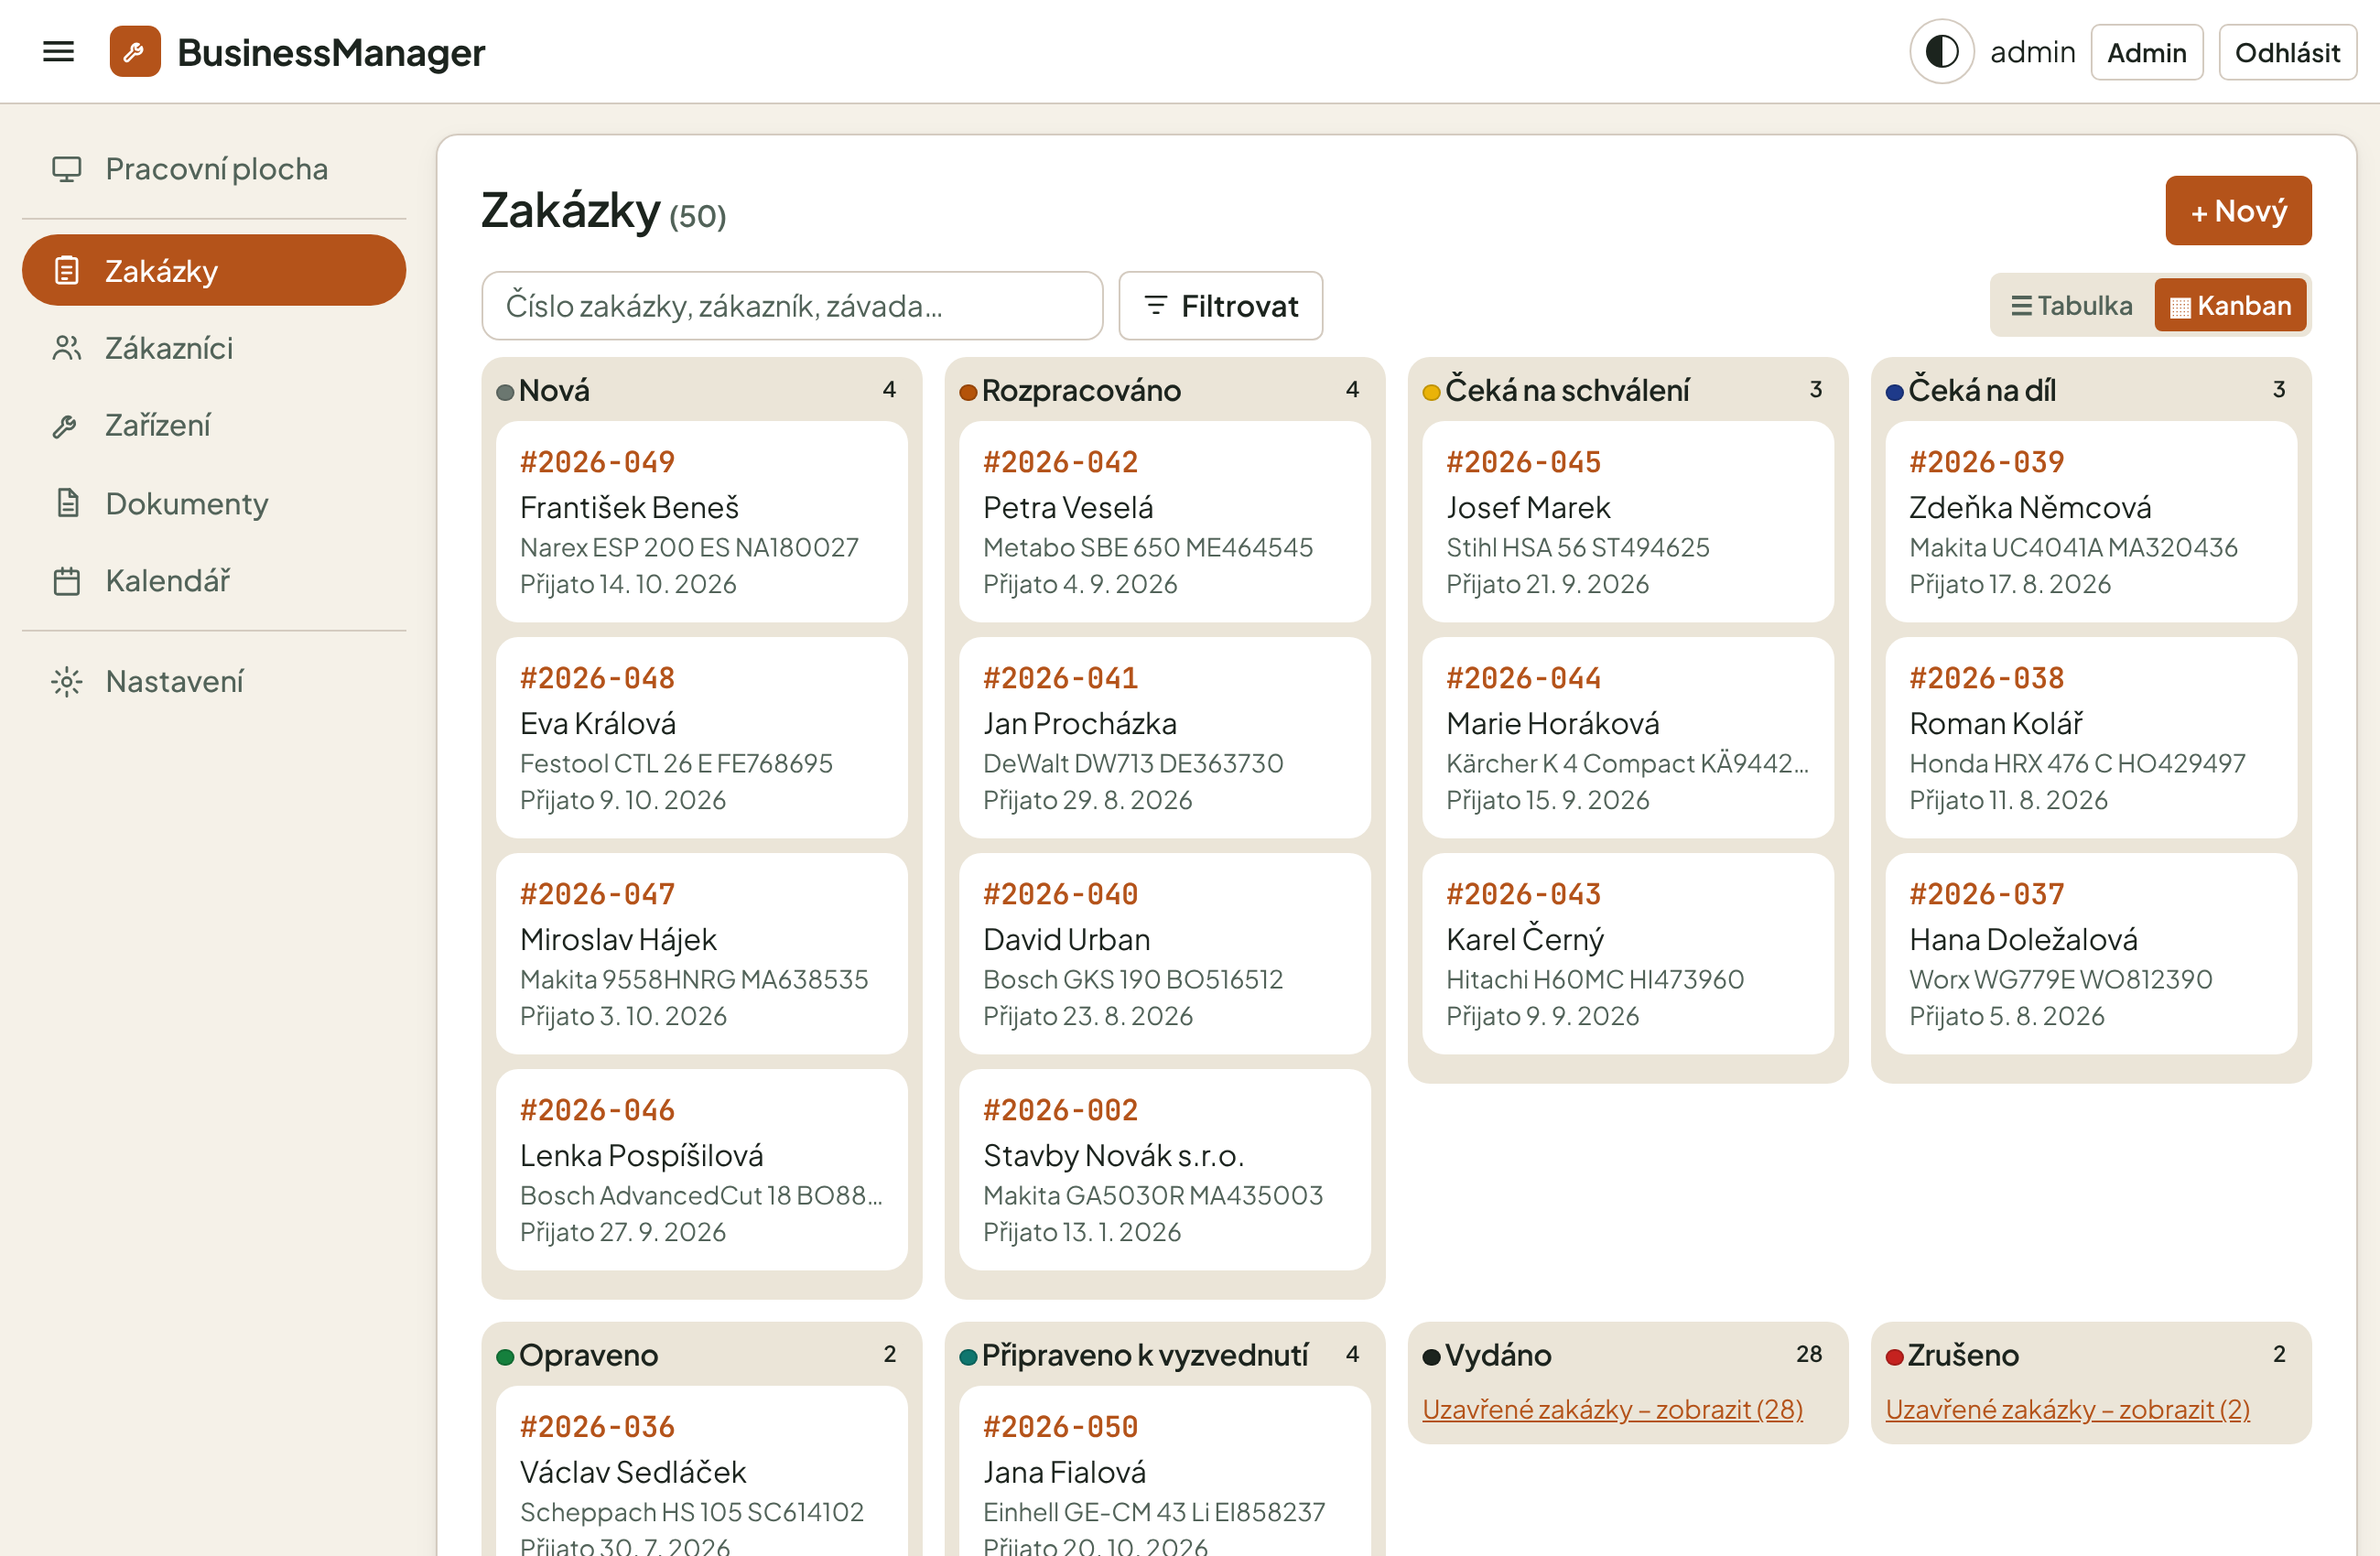
\includegraphics[width=\linewidth]{obrazky/navrh/bm-zakazky-kanban.png}
\caption{Kanbanové zobrazení zakázek v~aplikaci, sloupce odpovídají stavům zakázky, inspirováno Odoo (zdroj: vlastní)}\label{obr:bm-kanban}
\end{figure}

\subsection{Úpravy rozhraní podle doporučení}\label{sec:ui-upravy}

Při porovnání se zásadami vzniklo několik úprav a~všechny byly provedeny:
\begin{itemize}
\item Nastavení (údaje o~firmě, DPH, uživatelé, číselníky, šablony dokumentů, zálohování) bylo skryto a~zamčeno pro běžné zaměstnance. Později se rozdělení rozšířilo na role (Zaměstnanec, Technik, Administrativa, Administrátor): každý uživatel vidí jen tlačítka a~části aplikace, na které má oprávnění \cite{Nielsen-progressive}, \cite[s.~2331]{Sajedi2011}.
\item Styly Bootstrap a~knihovna htmx jsou přibaleny přímo do aplikace. Dříve se načítaly z~internetu a~bez připojení se aplikace zobrazila bez stylů, takže uživatel nevěděl, co se děje \cite{Nielsen-heuristiky}.
\item Při prvním spuštění provede aplikaci průvodce, který založí účet administrátora a~základní údaje o~firmě. Povinný je jen název organizace \cite{Nielsen-heuristiky}.
\item Na stránce zakázky bylo dříve osm stejně vypadajících tlačítek v~jedné řadě. Nyní zůstávají vpravo nahoře jen akce s~dokumenty (zakázkový list, nabídka, faktura, objednávka) a~tlačítka pro úpravu zakázky a~přidání práce, materiálu, fotografií a~příloh jsou v~záložkách, kterých se týkají. Plnou barvou je zvýrazněn jen doporučený další krok podle stavu zakázky, například zakázkový list u~nově přijaté zakázky, přidání práce u~rozpracované zakázky a~vytvoření nabídky a~poté faktury u~opravené zakázky. Je-li doporučeným krokem přidání práce, otevře se rovnou záložka Práce. Uživatel tak hned vidí, co má udělat dál \cite{Kaplan2021}, \cite{Shneiderman-pravidla}.
\item Na stránce zakázky byl dříve vpravo pevný panel prohlížeče dokumentů s~vlastní lištou tlačítek, který zabíral polovinu obrazovky i~tehdy, když uživatel žádný soubor neprohlížel. Nyní mají záložky celou šířku a~vejdou se do jedné řady. Fotografie, přílohy i~doklady se otevírají v~okně přes téměř celou obrazovku, ve kterém zůstalo jen stažení, tisk a~zavření, a~obrázek se přibližuje kolečkem myši. V~okně lze také porovnat dva soubory vedle sebe \cite{Nielsen-heuristiky}, \cite[s.~2332]{Sajedi2011}.
\item Údaje zařízení a~zákazníka se dříve upravovaly na samostatné stránce. Nyní tlačítko \enquote{Upravit} změní údaje přímo v~detailu na políčka a~tlačítka na \enquote{Uložit} a~\enquote{Zrušit}. Vedle údajů zařízení lze zobrazit fotografii nebo dokument z~jeho zakázek, například štítek s~typem a~sériovým číslem, takže je uživatel při přepisování nemusí držet v~paměti \cite{Shneiderman-pravidla}, \cite{Nielsen-heuristiky}.
\item Potvrzení nevratných akcí (například smazání) dříve zobrazoval systémový dialog prohlížeče s~adresou serveru. Nyní se zobrazí okno ve vzhledu aplikace se srozumitelnou otázkou a~tlačítkem, které říká, co se stane \cite{Shneiderman-pravidla}, \cite[s.~2331--2332]{Sajedi2011}.
\item Chybně zadaný e-mail nebo telefon dříve hlásila anglická bublina prohlížeče bez vysvětlení. Nyní formulář kontroluje server a~chybu ukáže česky u~políčka i~s~příkladem správného zápisu. Pole pro výběr souborů jsou také v~češtině \cite{Nielsen-heuristiky}.
\item Formuláře nové zakázky, nabídky a~faktury mají pod poli krátkou nápovědu, například že cena se zadává bez DPH a~DPH se dopočítá nebo že položky nabídky se převezmou ze zakázky \cite[s.~2330]{Sajedi2011}.
\end{itemize}
